\documentclass[12pt]{report}

\usepackage{cmap}
\usepackage[T2A]{fontenc}
\usepackage[utf8]{inputenc}
\usepackage[english,russian]{babel}

\usepackage{amssymb}

\usepackage{amsmath}

\usepackage{csquotes}

\includegraphics{}

\usepackage{longtable}

\usepackage{graphicx}
\usepackage{float}%"Плавающие" картинки
\usepackage{wrapfig}%Обтекание фигур (таблиц, картинок и прочего)
\graphicspath{{images/}}
\usepackage[usenames]{color}

\usepackage{listings}

\lstset{
language=haskell,                 % выбор языка для подсветки (здесь это Haskell)
basicstyle=\small\sffamily, % размер и начертание шрифта для подсветки кода
numbers=left,               % где поставить нумерацию строк (слева\справа)
numberstyle=\tiny,           % размер шрифта для номеров строк
stepnumber=1,                   % размер шага между двумя номерами строк
numbersep=5pt,                % как далеко отстоят номера строк от подсвечиваемого кода
showspaces=false,            % показывать или нет пробелы специальными отступами
showstringspaces=false,      % показывать или нет пробелы в строках
showtabs=false,             % показывать или нет табуляцию в строках
frame=single,              % рисовать рамку вокруг кода
tabsize=1,                 % размер табуляции по умолчанию равен 2 пробелам
captionpos=t,              % позиция заголовка вверху [t] или внизу [b] 
breaklines=true,           % автоматически переносить строки (да\нет)
breakatwhitespace=false, % переносить строки только если есть пробел
escapeinside={\#*}{*)}   % если нужно добавить комментарии в коде
}


% Для измененных титулов глав:
\usepackage{titlesec, blindtext, color} % подключаем нужные пакеты
\definecolor{gray75}{gray}{0.75} % определяем цвет
\newcommand{\hsp}{\hspace{20pt}} % длина линии в 20pt
% titleformat определяет стиль
\titleformat{\chapter}[hang]{\Huge\bfseries}{\thechapter\hsp\textcolor{gray75}{|}\hsp}{0pt}{\Huge\bfseries}


\usepackage{pgfplots}
\usepackage{filecontents}
\usetikzlibrary{datavisualization}
\usetikzlibrary{datavisualization.formats.functions}


\begin{filecontents}{Classic.dat}
	100 4.927
	200 45.956
	300 222.990
	400 1656.764
	500 4154.464
	600 8910.944
	700 16988.810
\end{filecontents}

\begin{filecontents}{Grape.dat}
	100 2.517
	200 22.215
	300 90.549
	400 268.980
	500 991.378
	600 5808.120
	700 11308.290
\end{filecontents}

\begin{filecontents}{Optymize_Grape.dat}
	100 0.049
	200 0.205
	300 0.479
	400 0.872
	500 1.371
	600 1.973
	700 2.866
\end{filecontents}

\begin{filecontents}{Classic_un.dat}
	101 5.150
	201 43.338
	301 281.546
	401 1865.899
	501 5668.476
	601 12540.691
	701 24528.664
\end{filecontents}

\begin{filecontents}{Grape_un.dat}
	101 2.368
	201 22.306
	301 88.246
	401 386.807
	501 1538.992
	601 7346.204
	701 14666.842
\end{filecontents}

\begin{filecontents}{Optymize_Grape_un.dat}
	101 0.049
	201 0.204
	301 0.491
	401 0.865
	501 1.409
	601 1.959
	701 2.877
\end{filecontents}



\begin{document}
	\begin{titlepage}
		\centering
		{\scshape\LARGE МГТУ им. Баумана \par}
		\vspace{3cm}
		{\scshape\Large Лабораторная работа №2\par}
		\vspace{0.5cm}	
		{\scshape\Large По курсу: "Анализ алгоритмов"\par}
		\vspace{1.5cm}
		{\huge\bfseries Оценка трудоемкости алгоритмов на примере алгоритмов умножения матриц\par}
		\vspace{2cm}
		{\Large Работу выполнил: Левушкин Илья, ИУ7-52Б\par}
		\vspace{0.5cm}
		{\Large Преподаватели:  Волкова Л.Л., Строганов Ю.В.\par}
		
		\vfill
		\large \textit {Москва, 2019} \par
	\end{titlepage}
	
	\tableofcontents
	
	\newpage
	\chapter*{Введение}
	
	~\
	
	\addcontentsline{toc}{chapter}{Введение}
	
	 \begin{displayquote}[Афоризм, рожденный из практики приема курсовых работ.]
	 	\textit{
	 Для решения любой сколь угодно простой задачи можно написать программу, которая будет работать сколь угодно медленно.
	}
	 \end{displayquote}
	
	Скорость выполнения программы (или производительность) зависят от многих факторов: языка программирования, способа реализации транслятора (компилятор, интерпретатор), производительности процессора. Поэтому заранее оценить производительность еще не написанной программы сложно. Но для уже разработанного алгоритма и написанной программы оценить перспективы ее использования с различными объемами данных вполне реально. Для этого и вводится понятие трудоемкости.
	
	\textbf{Трудоемкость программы (алгоритма)} – это зависимость количества массовых операций (сравнения, обмены, сдвиги, повторения цикла и т.п.) от объема (размерностей) обрабатываемых данных.
	
	Самое важное, что трудоемкость напрямую не связана со временем выполнения программы, но является мерой затрат на ее выполнение. Отметим наиболее важные свойства трудоемкости:
	\begin{itemize}
		\item трудоемкость определяется отдельно для каждого вида операций;
		\item трудоемкость может зависеть от входных данных. Поэтому оценка трудоемкости дается для лучшего и худшего случая, а также в среднем Tmin, Tmax, Tср . Свойство программы – иметь различную трудоемкость для разных данных, называется чувствительностью к данным;
		\item на практике обычно используется грубая оценка трудоемкости, основанная на понятии скорости (степени) роста функции.
	\end{itemize}
	
	Для грубой оценки трудоемкости есть свои основания. Дело в том, что размерности исходных данных \textbf{(N)} меняются в программах в широких пределах: на несколько порядков при отладке программы и ее работе в реальных условиях. Поэтому для функции трудоемкости важно ее асимптотическое поведение при достаточно больших \textbf{N}. Говорится, что функция  \textbf{T(N)} имеет степень роста  \textbf{G(N)}, если 
	 \begin{equation} \label{eq0}
	\exists C,N0 : \forall N>N0: C*G(N) > T(N)
	\end{equation}
	, то есть начиная с некоторого  \textbf{N0} функция  \textbf{G(N)} всегда превышает  \textbf{T(N)} с некотором коэффициентом пропорциональности.
	
	\begin{figure}[h!]
		\centering
		{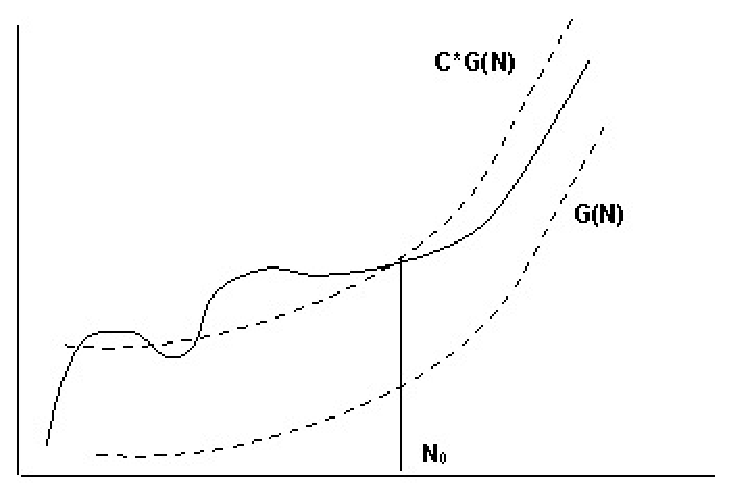
\includegraphics[width=1\linewidth]{1}}
		\caption{Определение степени роста функции T(N).}
		\label{ris:image1}
	\end{figure}
	
	
	 \vspace{0.5cm}
	 
	\textbf{Умножение матриц} — это один из базовых алгоритмов, который широко применяется в различных численных методах, и в частности в алгоритмах машинного обучения. Многие реализации прямого и обратного распространения сигнала в сверточных слоях неронной сети базируются на этой операции. Так порой до 90-95\% всего времени, затрачиваемого на машинное обучение, приходится именно на эту операцию. Почему так происходит? Ответ кроется в очень эффективной реализации этого алгоритма для процессоров, графических ускорителей (а в последнее время и специальных ускорителей матричного умножения). Матричное умножение — один из немногих алгоритмов, которые позволяет эффективно задействовать все вычислительные ресурсы современных процессоров и графических ускорителей. Поэтому не удивительно, что многие алгоритмы стараются свести к матричному умножению — дополнительная расходы, связанные с подготовкой данных, как правило с лихвой окупаются общим ускорением алгоритмов.
	
	Так как реализован алгоритм матричного умножения? На сколько сильно одни алгоритмы умножения матриц могут быть эффективней других алгоритмов? В данной лабораторной работе будут рассмотрены три различных алгоритма умножения матриц: стандартный, алгоритм Виноградова и его оптимизированная версия с последующей оценкой трудоемкости данных алгоритмов.
	
	\chapter{Цель}
	
	~\
	
	Целью данной лабораторной работы является изучение алгоритмов умножения матриц:
	\begin{itemize}
		\item стандартный;
		\item алгоритм Виноградова.
	\end{itemize}
	С последующей оценкой трудоемкости получившихся алгоритмов.
	
	\chapter{Задачи}
	
	~\
	
	Для достижение поставленной цели необходимо решить следующие \textbf{задачи}:
	\begin{itemize}
		\item проанализировать и разработать существующие реализации стандартного алгоритма и алгоритма Виноградова;
		\item также разработать оптимизированную версию алгоритма Виноградова;
		\item выбрать технологии для последующих реализаций и иследования
		алгоритмов;
		\item реализовать эти алгоритмы;
		\item произвести тестирование корректности работы реализаций;
		\item произвести оценку трудоемкости этих алгоритмов;
		\item сравнить быстродействие реализаций;
		\item описать и обосновать полученные результаты в отчете о выполненной лабораторной работе, выполненного как расчётно-пояснительная записка к работе.
	\end{itemize}
	
	
	\chapter{Аналитическая часть}
	
	\section{Определение}
	
	~\
	
	Пусть даны две прямоугольные матрицы ${\displaystyle A}$ и ${\displaystyle B}$ размерности ${\displaystyle l\times m}$ и ${\displaystyle m\times n}$ соответственно:
	
	
	\begin{equation} \label{eq1}
		A={
			\begin{bmatrix}
				a_{11} & a_{12} & \cdots & a_{1m} \\
				a_{21} & a_{22} & \cdots & a_{2m} \\
				\vdots & \vdots & \ddots & \vdots \\
				a_{l1} & a_{l2} & \cdots & a_{lm}
			\end{bmatrix}},
	    B={
	    	\begin{bmatrix}
		    	b_{11} & b_{12} & \cdots & b_{1n} \\
		    	b_{21} & b_{22} & \cdots & b_{2n} \\
		    	\vdots & \vdots & \ddots & \vdots \\
		    	b_{m1} & b_{m2} & \cdots & b_{mn}
	    	\end{bmatrix}
    }.
	\end{equation}
	
	Тогда матрица ${\displaystyle C}$ размерностью ${\displaystyle l\times n}$:
	
	\begin{equation} \label{eq2}
	C={
		\begin{bmatrix}
		c_{11} & c_{12} & \cdots & c_{1n} \\
		c_{21} & c_{22} & \cdots & c_{2n} \\
		\vdots & \vdots & \ddots & \vdots \\
		c_{l1} & c_{l2} & \cdots & c_{ln}
		\end{bmatrix}
	}
	\end{equation}
	
	в которой:
	
	\begin{equation} \label{eq3}
	{\displaystyle c_{ij}=
		\sum _{r=1}^{m}a_{ir}b_{rj}\;\;\;\left(i=1,2,\ldots l;\;j=1,2,\ldots n\right).}
	\end{equation}
	
	называется их произведением.
	
	Операция умножения двух матриц выполнима только в том случае, если число столбцов в первом сомножителе равно числу строк во втором; в этом случае говорят, что матрицы согласованы. В частности, умножение всегда выполнимо, если оба сомножителя — квадратные матрицы одного и того же порядка.
	
	Таким образом, из существования произведения ${\displaystyle AB}$ вовсе не следует существование произведения ${\displaystyle BA.}$.
	
	\section{Алгоритм Виноградова}
	
	~\
	
	Исходя из равенства \ref{eq2}, видно, что каждый элемент в нем представляет собой скалярное произведение соответствующих строки и столбца исходных матриц. Такое умножение допускает предварительную обработку, позволяющую часть работы выполнить заранее. ~\cite{Winograd}\\
	Рассмотрим два вектора U и V:
	
	\begin{equation}
	\label{u-def}
	U = A_{i} = (u_{1}, u_{2}, \ldots, u_{n}),
	\end{equation}
	где $U = A_{i}$ -- i-ая строка матрицы A,\\
	$u_{k} = a_{ik}, \overline{k = 1 \ldots n}$ -- элемент i-ой строки k-ого столбца матрицы A.\\
	
	\begin{equation}
	\label{v-def}
	V = B_{j} = (v_{1}, v_{2}, \ldots, v_{n}),
	\end{equation}
	где $V = B_{j}$ -- j-ый столбец матрицы B,\\
	$v_{k} = b_{kj}, \overline{k = 1 \ldots n}$ -- элемент k-ой строки j-ого столбца матрицы B.\\
	
	По определению их скалярное произведение равно:\\
	\begin{equation}
	\label{uv-def}
	U \cdot V = u_{1}v_{1} + u_{2}v_{2} + u_{3}v_{3} + u_{4}v_{4}.
	\end{equation}
	Равенство \ref{uv-def} можно переписать в виде:\\
	\begin{equation}
	\label{uv}
	U \cdot V = (u_{1} + v_{2})(u_{2} + v_{1}) + (u_{3} + v_{4})(u_{4} + v_{3}) - u_{1}u_{2} - u_{3}u_{4} - v_{1}v_{2} - v_{3}v_{4}.
	\end{equation}
	В равенстве \ref{uv-def} насчитывается 4 операции умножения и 3 операции сложения, в равенстве \ref{uv} насчитывается 6 операций умножения и 9 операций сложения. Однако выражение $- u_{1}u_{2} - u_{3}u_{4}$ используются повторно при умножении i-ой строки матрицы A на каждый из столбцов матрицы B, а выражение $- v_{1}v_{2} - v_{3}v_{4}$ - при умножении j-ого столбца матрицы B на строки матрицы A. Таким образом, данные выражения можно вычислить предварительно для каждых строк и столбцов матриц для сокращения повторных вычислений. В результате повторно будут выполняться лишь 2 операции умножения и 7 операций сложения (2 операции нужны для добавления предварительно посчитанных произведений).
	
	\subsection{Оптимизированный алгоритм Винограда}\label{optymize}
	
	~\
	
	Для оптимизации алгоритма Винограда могут использоваться такие стратегии, как:
	\begin{itemize}
		\item предварительные вычисления повторяющихся одинаковых действий;
		\item использование более быстрых операций при вычислении (такие, как смещение битов вместо умножения или деления на 2);
		\item уменьшения количества повторных проверок;
		\item использование аналогичных конструкций, уменьшающих трудоёмкость операций (к примеру, замена сложения с 1 на инкремент).
	\end{itemize}
	Ниже представлен список личностей, проводивших оптимизацию алгоритма:
	\begin{itemize}
		\item в 2010 Эндрю Стотерс усовершенствовал алгоритм до $O(n^{2.374})$;
		\item в 2011 году Вирджиния Уильямс усовершенствовала алгоритм до $O(n^{2.3728642})$;
		\item в 2014 году Франсуа Ле Галль упростил метод Уильямса и получил новую улучшенную оценку $O(n^{2.3728639})$.
	\end{itemize}
	
	\subsection{Модель вычислений}\label{model}
	
	~\
	
	В рамках данной работы используется следующая модель вычислений:
	\begin{itemize}
		\item операции, имеющие трудоемкость 1: $<$, $>$, $=$, $<=$, $=>$, $==$, $!=$,$+$, $-$, $\ast$, /, $+$=, $-$=, $\ast$=, $/$=, [ ];
		\item оператор условного перехода имеет трудоёмкость, равную трудоёмкости операторов тела условия;
		\item оператор цикла for имеет трудоемкость:
		\begin{equation}
		\label{for_cost}
		F_{for} = F_{init} + F_{check} + N \ast (F_{body} + F_{inc} + F_{check}),
		\end{equation}
		где $F_{init}$ -- трудоёмкость инициализации, $F_{check}$ -- трудоёмкость проверки условия, $F_{inc}$ -- трудоёмкость инкремента аргумента, $F_{body}$ -- трудоёмкость операций в теле цикла, $N$ -- число повторений. ~\cite{AlgAnalysis}
	\end{itemize} 
	
	\section{Выводы по аналитической части}
	
	~\
	
	В рамках данной работы были выбраны для исследования стандартный алгоритм, алгоритм Виноградова, а также оптимизированная его версия, умножения матриц.
	Были расписаны способы оптимизации алгоритма Винограда (\ref{optymize}) и выбрана модель вычислений по которой будет оцениваться трудоемкость алгоритмов (\ref{model}).
		
	\chapter{Конструкторская часть}
	
	\section{Реализация алгоритмов}
	
	\subsection{Стандартный алгоритм}
	
	~\
	
	В стандартном алгоритме мы перемножаем каждый вектор-строку первой матрицы на каждый вектор-столбец второй матрицы. То есть в первом цикле мы проходимся по всем строкам первой матрицы, во втором цикле проходимся по всем столбцам второй матрицы, и в третьем цикле мы проходимся по всем столбцам первой/строкам второй матрицы. При этом используем формулу \ref{eq3} для получения ответа.
	
	\subsection{Алгоритм Виноградова}
	
	~\
	
	В алгоритме Виноградова мы также пермножаем каждый вектор-строку первой матрицы на каждый вектор-столбец второй матрицы, только вместо того, чтобы делать это по отдельности, для каждого $i$-ого элемента: $u_{i}v_{i}$, мы считаем сумму сразу по 2 элемента: $u_{i}v_{i} + u_{i + 1}v_{i + 1}$. Преобразовав это выражение к: $(u_{i} + v_{i + 1})(u_{i + 1} + v_{i}) - u_{i}u_{i + 1} - v_{i}v_{i + 1}$, и посчитав $- u_{i}u_{i + 1} - v_{i}v_{i + 1}$ заранее (вне основного цикла), получим всего 1 операцию умножения и 2 операции сложения заместо двух операций умножения и одной операции сложения.
	
	\subsection{Список оптимизаций алгоритма Виноградова}
	
	~\
	
	Алгоритм Винограда был оптимизирован с помощью следующих модификаций:
	\begin{itemize}
		\item вычисление повторно используемых величин выполняется предварительно ($N / 2$, $N - 1$, $2 * k$);
		\item проверка на четность/нечетность матрицы происходит до основого цикла, и в зависимости от результата выбирается один из основных циклов: для четной и нечетной матрицы (цикл вычислений для нечётных элементов включён в основной цикл, добавив дополнительные операции). Данная модификация исключает повторные проверки на нечётность $N$;
		\item вместо обращения к $ij$-ому элементу массива результирующей матрицы на каждой итерации, в основном цикле используется указатель на $i$-ый элемент массива, чтобы во втором цикле исключить лишнее обращение к $i$-ому элементу массива;
		\item используется буфер buf для уменьшения количества обращений к результирующей матрице.
	\end{itemize}

   %используется список в списке, в который на каждой итерации добавляется результирующий элемент в его голову. Так как нам не нужно обращаться к конкретному элементу двумерного массива, а лишь к голове списка, это значительно ускоряет работу программы.
	\section{Схемы алгоритмов}
	
	~\
	
	На рисунках ~\ref{ris:image2}, ~\ref{ris:image3}, ~\ref{ris:image4}, ~\ref{ris:image5}, ~\ref{ris:image6}, ~\ref{ris:image7}, ~\ref{ris:image8}, ~\ref{ris:image9}, ~\ref{ris:image10} представлены схемы реализаций стандартного алгоритма, алгоритма Винограда и его оптимизированный вариант.
	
	\begin{figure}[H]
		\centering
		\includegraphics[width=1.2\linewidth]{Standard}
		\caption{Алгоритм умножения матриц.}
		\label{ris:image2}
	\end{figure}

\newpage

	\begin{figure}[H]
		\centering
		\includegraphics[width=0.8\linewidth]{Standard_sub}
		\caption{Подпрограмма стандартного умножения матриц.}
		\label{ris:image3}
	\end{figure}

\newpage

\begin{figure}[H]
	\centering
	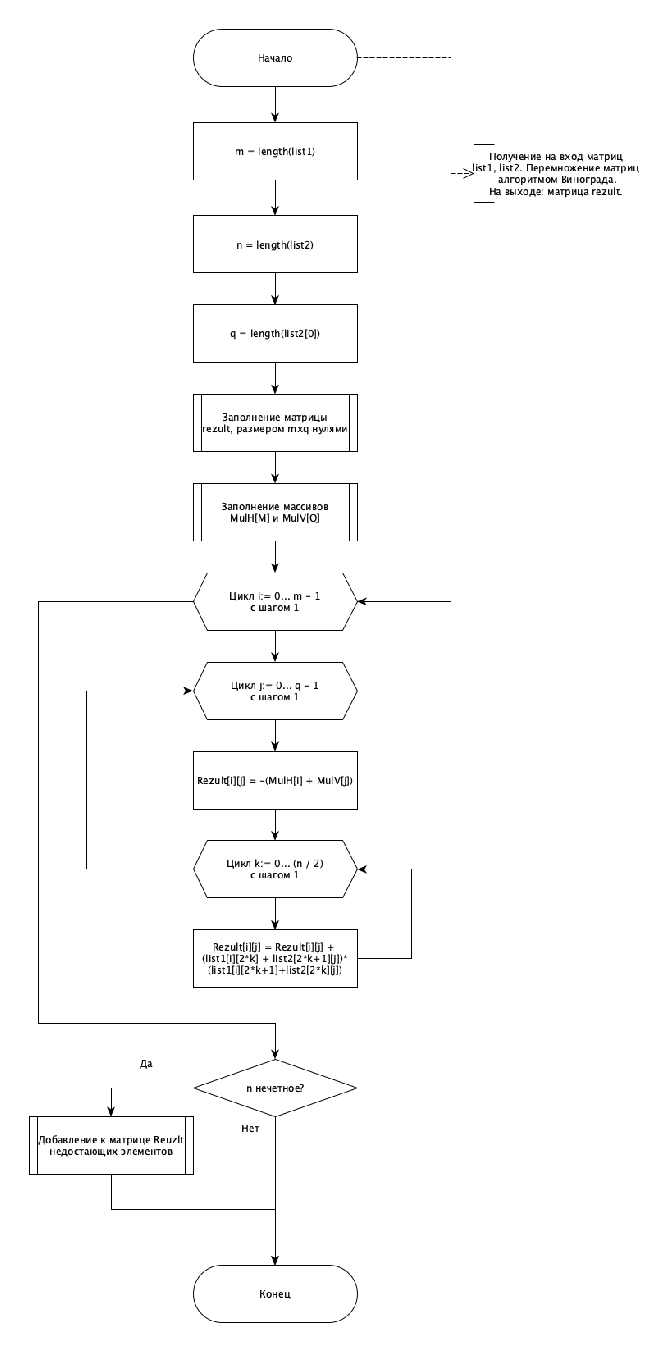
\includegraphics[width=0.75\linewidth]{Grape_sub}
	\caption{Подпрограмма умножения матриц по Винограду.}
	\label{ris:image4}
\end{figure}

\newpage

\begin{figure}[H]
	\centering
	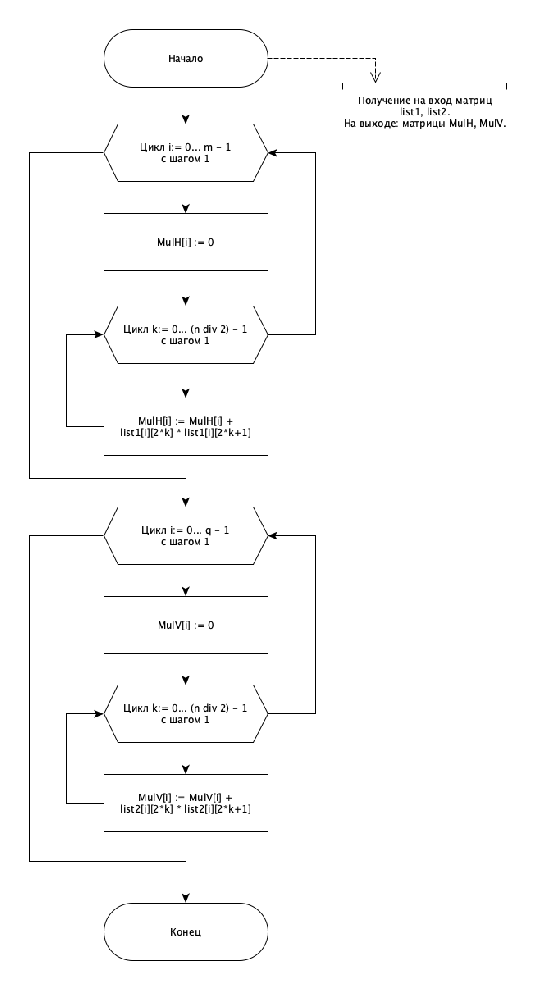
\includegraphics[width=0.8\linewidth]{Grape_MulHV}
	\caption{Подпрограмма заполнения массивов MulH[M] и MulV[Q].}
	\label{ris:image5}
\end{figure}

\newpage

\begin{figure}[H]
	\centering
	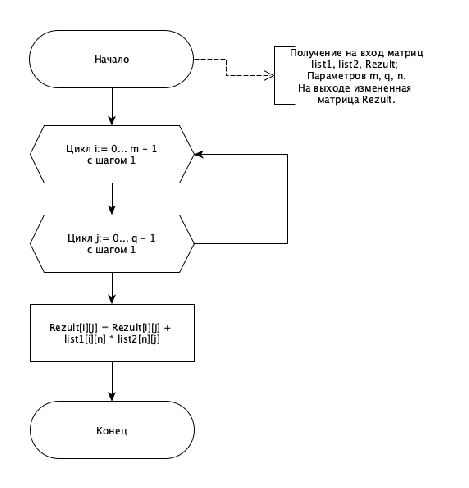
\includegraphics[width=0.8\linewidth]{Grape_nechet}
	\caption{Подпрограмма добавления к матрице Rezult нечетных элементов.}
	\label{ris:image6}
\end{figure}

\newpage

\begin{figure}[H]
	\centering
	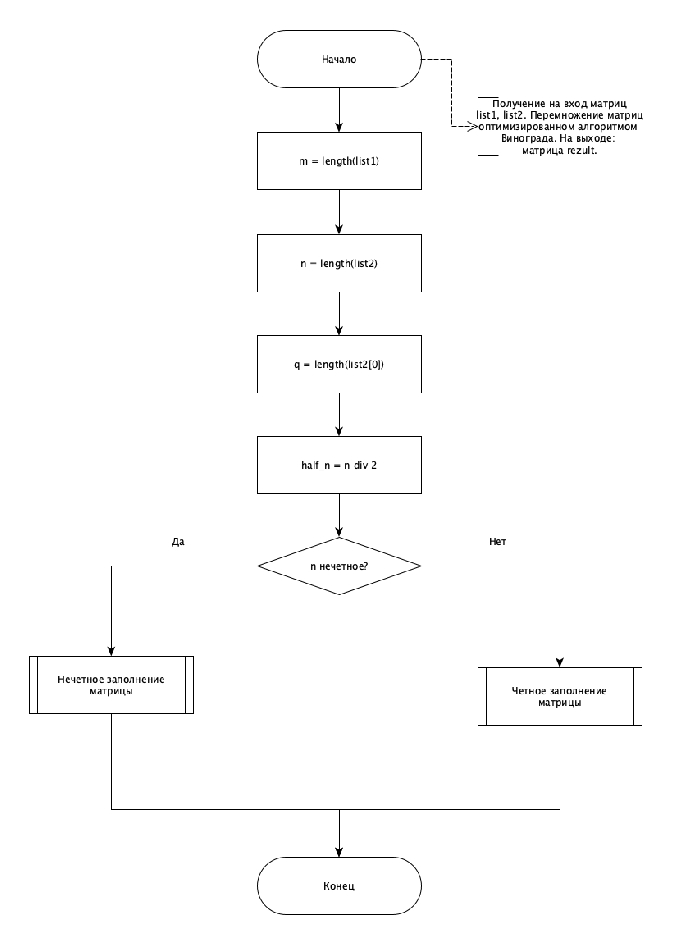
\includegraphics[width=0.8\linewidth]{Optymize_grape}
	\caption{Подпрограмма умножения матриц по Винограду (оптимизированный вариант).}
	\label{ris:image7}
\end{figure}

\newpage

\begin{figure}[H]
	\centering
	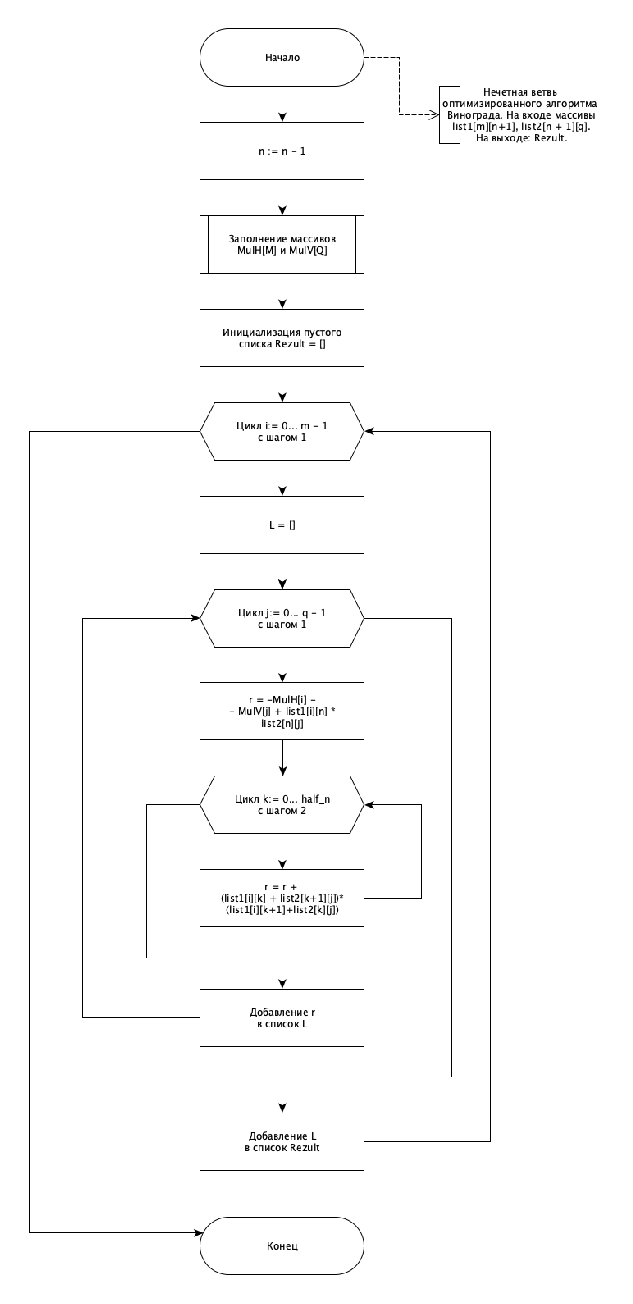
\includegraphics[width=0.75\linewidth]{uneven}
	\caption{Подпрограмма нечетного заполнения матрицы.}
	\label{ris:image8}
\end{figure}

\newpage

\begin{figure}[H]
	\centering
	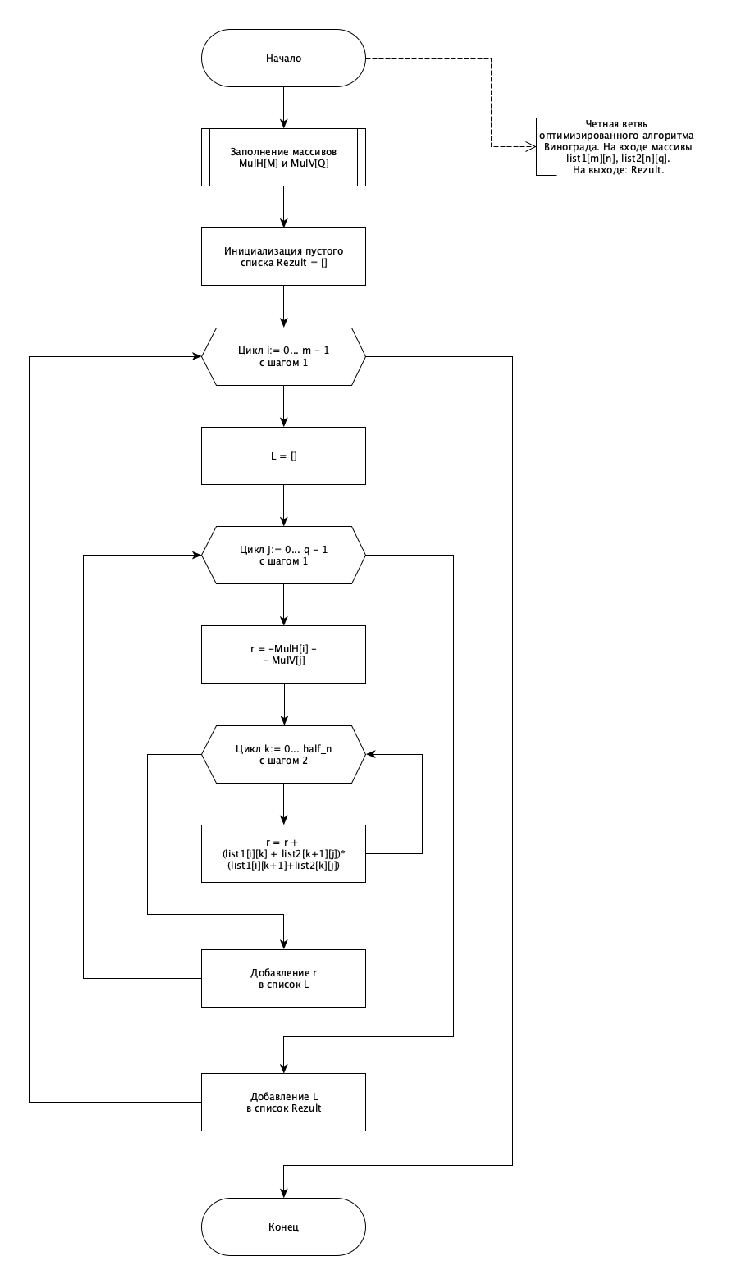
\includegraphics[width=0.8\linewidth]{even}
	\caption{Подпрограмма четного заполнения матрицы.}
	\label{ris:image9}
\end{figure}

\newpage

\begin{figure}[H]
	\centering
	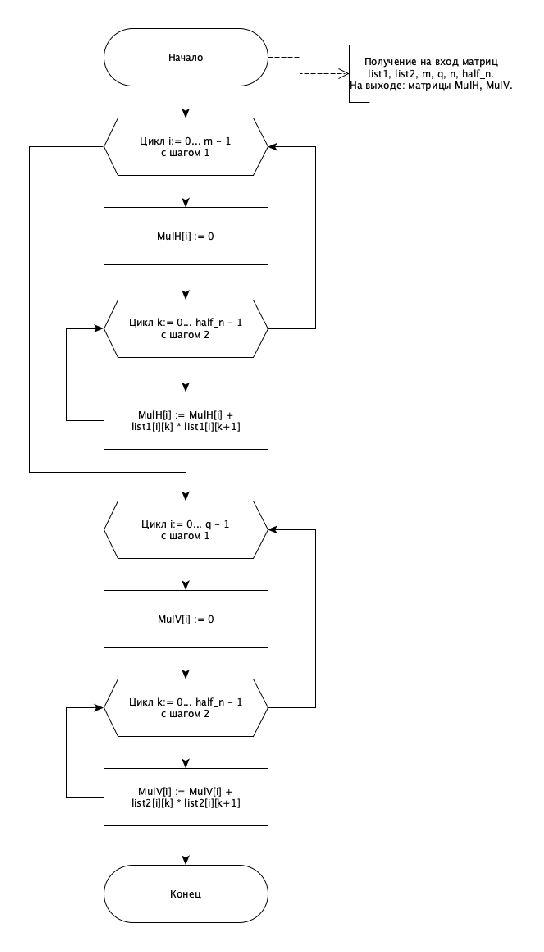
\includegraphics[width=0.8\linewidth]{optymize_grape_MulHV}
	\caption{Подпрограмма заполнения массивов MulH[M] и MulV[Q].}
	\label{ris:image10}
\end{figure}

	\section{Оценка трудоемкости}
	\subsection{Классический алгоритм}
	\begin{equation}
	\label{complex_classic}
	f_{classic} = 13MNQ + 4MQ + 4M + 1
	\end{equation}
	
	\subsection{Алгоритм Виноградова}
	
	~\
	
	Трудоёмкости составных частей алгоритма:
	\begin{itemize}
		\item цикл создания вектора MulH: $f_{I} = \frac{15}{2}MN + 4M + 2$;
		\item цикл создания вектора MulV:  $f_{II} = \frac{15}{2}NQ + 4Q + 2$;
		\item основной цикл: $f_{III} = 13MNQ + 4MQ + 4M + 2$;
		\item условный переход при чётном $N$: $f_{IV} = 2$;
		\item условный переход и цикл при нечётном $N$: $f_{IV} = 17MQ + 4M + 4$.
	\end{itemize}
	Общая трудоемкость алгоритма:
	\begin{itemize}
		\item при чётном $N$:
		\begin{equation}
		\label{complex_vin_even1}
		f_{vin} = f_{I} + f_{II} + f_{III} + f_{IV} = 13MNQ + \frac{15}{2}MN + \frac{15}{2}NQ + 4MQ + 8M + 4Q + 8
		\end{equation}
		\item при нечётном $N$:
		\begin{equation}
		\label{complex_vin_odd1}
		f_{vin} = f_{I} + f_{II} + f_{III} + f_{IV} = 13MNQ + \frac{15}{2}MN + \frac{15}{2}NQ + 21MQ + 12M + 4Q + 10
		\end{equation}
	\end{itemize}
	
	\subsection{Оптимизированный алгоритм Винограда}
	
	~\
	
	Трудоёмкости составных частей алгоритма:
	\begin{itemize}
		\item цикл создания вектора MulH: $f_{I} = \frac{11}{2}MN + 4M + 2$;
		\item цикл создания вектора MulV:  $f_{II} = \frac{11}{2}NQ + 4Q + 2$;
		\item основной цикл при чётном $N$: $f_{III} = 10MNQ + 17MQ + 4M + 6$;
		\item основной цикл при нечётном $N$: $f_{III} = 10MNQ + 10NQ + 4M + 2$.
	\end{itemize}
	Общая трудоемкость алгоритма:
	\begin{itemize}
		\item при чётном $N$:
		\begin{equation}
		\label{complex_vin_even2}
		f_{opt} = f_{I} + f_{II} + f_{III} = 10MNQ + \frac{11}{2}MN + \frac{11}{2}NQ + 9MQ + 8M + 4Q + 6
		\end{equation}
		\item при нечётном $N$:
		\begin{equation}
		\label{complex_vin_odd2}
		f_{opt} = f_{I} + f_{II} + f_{III} = 10MNQ + \frac{11}{2}MN + \frac{11}{2}NQ + 16MQ + 8M + 4Q + 10
		\end{equation}
	\end{itemize}
	
	
	\section{Замер используемой памяти}
	
	~\
	
	Пусть даны две матрицы $A$ и $B$ размерностью $M\times N$ и размерностью $N \times Q$ соответственно и для хранения целого числа требуется 4 байта памяти.
	
	В каждом из алгоритмов требуется хранить исходные матрицы $A$ и $B$ и матрицу результата умножения $C$, которая имеет размеры $M \times Q$. Таким образом, под хранение матриц требуется $4 \cdot (MN + NQ + MQ)$ байт памяти.
	
	Для алгоритма Винограда и его оптимизированного варианта требуется также хранить два дополнительных вектора $MulH$ и $MulV$. Их размеры $M$ и $Q$ соответственно, следовательно требуется дополнительно $4 \cdot (M + Q)$ байт памяти. В итоге для алгоритмов Винограда требуется $4 \cdot (MN + NQ + MQ + M + Q)$ байт памяти. Таким образом, при больших размерах матриц (больше 100) алгоритмы Винограда будут незначительно проигрывать по памяти классическому алгоритму.
	
	\section{Требования к программе}
	
	~\
	
	\begin{itemize}
		\item Программа должна предоставлять доступный и понятный интерфейс с выбором алгоритмов (и всех их реализаций);
		\item Должно быть 2 реализации алгоритма Виноградова:
		\begin{itemize}
			\item неоптимизированная;
			\item оптимизированная.
		\end{itemize}
		\item На вход каждой функции, реализующей конкретный алгоритм, подаются две матрицы {\bf целых} чисел;
		\item Пользователь должен иметь возможность вводить матрицы вручную либо выбрать пункт случайного заполнения, в случае чего ему будет предоставлен выбор длин матриц;	
		\item Требования к выводу программы:
		\begin{itemize}
			\item программа должна выдавать корректное перемножение двух матриц (см. Аналитискую часть);
			\item при вводе пустых матриц - программа не должна аварийно завершаться, а выдавать пустую матрицу;
			\item при вводе матриц, не удовлетворяющих условиям перемножения матриц (см. Аналитическую часть) - программа не должна аварийно завершаться, а выдавать пустую матрицу;
		\end{itemize}
	\end{itemize}
	
	
	\section{Выводы по конструкторской части}
	
	~\
	
	В результате проведенной работы было расписано описание алгоритмов, разработаны схемы алгоритмов, была оценена трудоемкость каждого из алгоритмов, а также расписаны оптимизации для алгоритма Винограда.
	
	Помимо всего прочего, был произведен замер используемой памяти программой (аналитически). Были сформулированы основные требования к программе.
	
	\chapter{Технологическая часть}
	
	\section{Средства реализации}
	
	~\
	
	Для реализации программы был использован язык программирования {\bf Haskell} ~\cite{Haskell}.
	Время работы алгоритмов было замерено с помощью функции {\bf getCPUTime} из библиотеки {\bf System.CPUTime}. Для отключения встроенной оптимизиации компилятора был использован атрибут -O0 компилятора ghci.
	Тестирование было организовано с помощью библиотеки  \textbf{TestHUnit}.
	При сравнении результатов двух функций использовалась функция randomRs из библиотеки System.Random, которая генерирует случайный список целых чисел нужного размера.
	
	\section{Сведения о модулях программы}
	
	~\
	
	Программа состоит из:
	\begin{itemize}
		\item Main.hs - Главный файл программы, в котором располагается меню;
		\item Lib.hs - файл с подключенными модулями реализаций алгоритмов;
		\item Standard.hs - Файл с реализацией стандартного алгоритма умножения матриц;
		\item Grape.hs - Файл с реализацией алгоритма Виноградова;
		\item Optymize\_grape.hs - Файл с реализацией оптимизированного алгоритма Виноградова;
		\item Spec.hs - Файл с модульными тестами.
	\end{itemize}
	
	{\bf Ниже приведены листинги  ~\ref{some-code1}, ~\ref{some-code2}, ~\ref{some-code3} функций программы.}
	
	\begin{lstlisting}[label=some-code1,caption=Стандартный алгоритм умножения матриц]
	
	import Data.List
	
	
	answer_fill :: Int -> Int -> [[Int]]
	answer_fill 0 j = []
	answer_fill i j = take j (repeat 0) : answer_fill (i - 1) j
	
	
	--c[m][q] += a[m][n] * b[n][q]
	get_new_line_answer :: Int -> Int -> Int -> [Int] -> [Int]
	get_new_line_answer j a b line = (take j line) ++ 
	([(line !! j) + a * b]) ++
	(reverse (take (length line - j - 1) $ reverse line))
	
	
	
	third_loop :: [Int] -> [[Int]] -> Int -> Int -> Int -> Int -> [[Int]] -> [[Int]]
	third_loop list1_i list2 i j k n answer | k == n    = answer
	| otherwise = 
	(third_loop list1_i list2 i j (k + 1) n $ 
	take i answer ++ 
	[get_new_line_answer j  
	(list1_i !! k)  
	((list2 !! k) !! j)
	(answer !! i)] ++ 
	(reverse (take (length answer - i - 1) $ reverse answer)))
	
	
	second_loop :: [Int] -> [[Int]] -> Int -> Int -> Int -> [[Int]] -> [[Int]]
	second_loop list1_i list2 i j q answer | j == q    = answer
	| otherwise = 
	second_loop list1_i list2 i (j + 1) q $
	third_loop list1_i list2 i j 0 (length list2) answer
	
	
	first_loop :: [[Int]] -> [[Int]] -> Int -> Int -> [[Int]] -> [[Int]]
	first_loop list1 list2 i m answer | i == m    = answer
	| otherwise = 
	first_loop list1 list2 (i + 1) m $
	second_loop (list1 !! i) list2 i 0 (length $ head list2) answer
	
	
	calc_multypl :: [[Int]] -> [[Int]] -> [[Int]]
	calc_multypl list1 list2 = (first_loop list1 list2 0 (length list1)) $ answer_fill
	(length list1)  (length $ head list2)
	
	
	check_size :: [[Int]] -> Int -> Int
	check_size list 1 = length list
	check_size list 2 = length $ head list
	
	
	check_matr :: [[Int]] -> Bool
	check_matr [] = True
	check_matr (_:[]) = True
	check_matr (x:xs) = if ((length x) == (length $ head xs))
	then check_matr xs
	else False
	
	
	standard :: [[Int]] -> [[Int]] -> [[Int]]
	standard list1 list2 = if (check_matr list1 && check_matr list2) 
	then (if (check_size list1 2) == (check_size list2 1)
	then calc_multypl list1 list2 
	else [[]])
	else [[]]
	\end{lstlisting}
	
	\begin{lstlisting}[label=some-code2,caption=Алгоритм Виноградова]
	import Data.List
	
	answer_fill :: Int -> Int -> [[Int]]
	answer_fill 0 j = []
	answer_fill i j = take j (repeat 0) : answer_fill (i - 1) j
	
	
	
	mulh_loop :: Int -> Int -> Int -> [Int] -> Int -> Int
	mulh_loop i k n a_i mulh_i | k == div n 2    = mulh_i
	| otherwise       = mulh_i + (a_i !! (2 * k)) * (a_i !! (2 * k + 1)) +
	(mulh_loop i (k + 1) n a_i mulh_i)
	
	
	
	calc_mulh :: Int -> Int -> Int -> [[Int]] -> [Int] -> [Int]
	calc_mulh i m n list mulh | i == m    = mulh
	| otherwise = calc_mulh (i + 1) m n list 
	((take i mulh) ++
	[mulh_loop i 0 n (list !! i) (mulh !! i)] ++
	(reverse (take (length mulh - i - 1) $ reverse mulh)))
	
	
	
	mulv_loop :: Int -> Int -> Int -> [[Int]] -> Int -> Int
	mulv_loop i k n a mulv_i   | k == div n 2    = mulv_i
	| otherwise       = mulv_i + ((a !! (2 * k)) !! i) * ((a !! (2 * k + 1)) !! i) +
	(mulv_loop i (k + 1) n a mulv_i)
	
	
	
	calc_mulv :: Int -> Int -> Int -> [[Int]] -> [Int] -> [Int]
	calc_mulv i q n list mulv | i == q    = mulv
	| otherwise = calc_mulv (i + 1) q n list 
	((take i mulv) ++
	[mulv_loop i 0 n list (mulv !! i)] ++
	(reverse (take (length mulv - i - 1) $ reverse mulv)))
	
	
	main_k_loop :: [[Int]] -> [[Int]] -> Int -> Int -> Int -> [[Int]] -> [[Int]]
	main_k_loop a b i j k c | k == div (length b) 2 = c
	| otherwise             = main_k_loop a b i j (k + 1) (
	(take i c) ++
	[
	take j (c !! i) ++
	[((c !! i) !! j) + ((((a !! i) !! (2 * k)) + ((b !! (2 * k + 1)) !! j)) * 
	(((a !! i) !! (2 * k + 1)) + ((b !! (2 * k)) !! j)))] ++
	(reverse (take (length (c !! i) - j - 1) $ reverse (c !! i)))
	] ++
	(reverse (take (length c - i - 1) $ reverse c))
	)
	
	
	
	main_q_loop :: [[Int]] -> [[Int]] -> [Int] -> [Int] -> Int -> Int -> [[Int]] -> [[Int]]
	main_q_loop a b mulh mulv i j c | j == (length $ head b)  = c
	| otherwise               = main_q_loop a b mulh mulv i (j + 1) (main_k_loop a b i j 0 
	(
	(take i c) ++
	[
	take j (c !! i) ++
	[-1 * ((mulh !! i) + (mulv !! j))] ++
	(reverse (take (length (c !! i) - j - 1) $ reverse (c !! i)))
	] ++
	(reverse (take (length c - i - 1) $ reverse c))
	)
	)
	
	
	main_calc :: [[Int]] -> [[Int]] -> [Int] -> [Int] -> Int -> [[Int]] -> [[Int]]
	main_calc a b mulh mulv i c | i == (length a)  = c
	| otherwise        = main_calc a b mulh mulv (i + 1) (main_q_loop a b mulh mulv i 0 c)
	
	
	
	nechet_q_loop :: [[Int]] -> [[Int]] -> Int -> Int -> Int -> Int -> [[Int]] -> [Int]
	nechet_q_loop a b i j n q c | j == q    = (c !! i)
	| otherwise = nechet_q_loop a b i (j + 1) n q 
	(
	(take i c) ++ 
	[(take j (c !! i)) ++
	[((c !! i) !! j) + ((a !! i) !! (n - 1)) * ((b !! (n - 1)) !! j)] ++ 
	(reverse (take (length (c !! i) - j - 1) $ reverse (c !! i)))] ++
	(reverse (take (length c - i - 1) $ reverse c))
	)
	
	
	
	nechet_m_loop :: [[Int]] -> [[Int]] -> Int -> Int -> Int -> Int -> [[Int]] -> [[Int]]
	nechet_m_loop a b i m q n c | i == m    = c
	| otherwise = nechet_m_loop a b (i + 1) m q n
	((take i c) ++
	[nechet_q_loop a b i 0 n q c] ++
	(reverse (take (length c - i - 1) $ reverse c)))
	
	
	nechet_calc :: [[Int]] -> [[Int]] -> Int -> Int -> Int -> [[Int]] -> [[Int]]
	nechet_calc a b m q n c | not (odd n) = c
	| otherwise   = nechet_m_loop a b 0 m q n c
	
	
	
	calc_multypl :: [[Int]] -> [[Int]] -> [[Int]]
	calc_multypl list1 list2 = nechet_calc list1 list2 (length list1)
	(length $ head list2)
	(length list2) $ 
	main_calc list1 list2 
	(calc_mulh 0 (length list1) (length $ head list1) list1 (take (length list1) (repeat 0)))
	(calc_mulv 0 (length $ head list2) (length list2) list2 (take (length $ head list2) (repeat 0)))
	0
	(answer_fill (length list1) (length $ head list2))
	
	
	
	check_size :: [[Int]] -> Int -> Int
	check_size list 1 = length list
	check_size list 2 = length $ head list
	
	
	check_matr :: [[Int]] -> Bool
	check_matr [] = True
	check_matr (_:[]) = True
	check_matr (x:xs) = if ((length x) == (length $ head xs))
	then check_matr xs
	else False
	


	grape :: [[Int]] -> [[Int]] -> [[Int]]
	grape list1 list2 = if (check_matr list1 && check_matr list2) 
	then (if (check_size list1 2) == (check_size list2 1)
	then calc_multypl list1 list2 else [[]])
	else [[]]
	\end{lstlisting}
	
	\begin{lstlisting}[label=some-code3,caption=Оптимизированный алгоритм Виноградова]
	answer_fill :: Int -> Int -> [[Int]]
	answer_fill 0 j = []
	answer_fill i j = take j (repeat 0) : answer_fill (i - 1) j
	
	
	
	
	mulh_loop :: Int -> Int -> Int -> [Int] -> Int -> Int
	mulh_loop i k n a_i mulh_i | k >= n    = mulh_i
	| otherwise = mulh_i + (a_i !! k) * (a_i !! (k + 1)) + 
	(mulh_loop i (k + 2) n a_i mulh_i)
	
	
	
	calc_mulh :: Int -> Int -> Int -> [[Int]] -> [Int] -> [Int]
	calc_mulh i m n list mulh | i == m    = mulh
	| otherwise = calc_mulh (i + 1) m n list 
	((take i mulh) ++
	[mulh_loop i 0 n (list !! i) (mulh !! i)] ++
	(reverse (take (length mulh - i - 1) $ reverse mulh)))
	
	
	
	mulv_loop :: Int -> Int -> Int -> [[Int]] -> Int -> Int
	mulv_loop i k n a mulv_i   | k >= n      = mulv_i
	| otherwise   = mulv_i + ((a !! k) !! i) * ((a !! (k + 1)) !! i) + 
	(mulv_loop i (k + 2) n a mulv_i)
	
	
	
	calc_mulv :: Int -> Int -> Int -> [[Int]] -> [Int] -> [Int]
	calc_mulv i q n list mulv | i == q    = mulv
	| otherwise = calc_mulv (i + 1) q n list 
	((take i mulv) ++
	[mulv_loop i 0 n list (mulv !! i)] ++
	(reverse (take (length mulv - i - 1) $ reverse mulv)))
	
	
	
	
	buf :: [Int] -> [[Int]] -> Int -> Int -> Int -> Int
	buf a_i b j k n | k >= n    = 0
	| otherwise = (((a_i !! k) + ((b !! (k + 1)) !! j)) * 
	((a_i !! (k + 1)) + ((b !! k) !! j))) + 
	(buf a_i b j (k + 2) n)
	
	
	
	main_q_loop :: [Int] -> [[Int]] -> Int -> Int -> Int -> Int -> Int -> [Int] -> [Int]
	main_q_loop a_i b j m q n mulh_i mulv | j == q    = []
	| otherwise = ((buf a_i b j 0 n) - 
	(mulh_i + 
	(mulv !! j))) : 
	(main_q_loop a_i b (j + 1) m q n mulh_i mulv)
	
	
	main_calc :: [[Int]] -> [[Int]] -> Int -> Int -> Int -> Int -> [Int] -> [Int] -> [[Int]]
	main_calc a b i m q n mulh mulv | i == m    = []
	| otherwise = (main_q_loop (a !! i) b 0 m q n (mulh !! i) mulv) : 
	(main_calc a b (i + 1) m q n mulh mulv)
	
	
	buf_nechet :: [Int] -> [[Int]] -> Int -> Int -> Int -> Int
	buf_nechet a_i b j k n_minus_one | k >= n_minus_one = 0
	| otherwise        = (((a_i !! k) + ((b !! (k + 1)) !! j)) * 
	((a_i !! (k + 1)) + ((b !! k) !! j))) + 
	(buf_nechet a_i b j (k + 2) n_minus_one)
	
	
	
	add_nechet :: [Int] -> [[Int]] -> Int -> Int -> Int
	add_nechet a_i b j n_minus_one = (a_i !! n_minus_one) * ((b !! n_minus_one) !! j)
	
	
	
	main_q_loop_nechet :: [Int] -> [[Int]] -> Int -> Int -> Int -> Int -> Int -> [Int] -> Int -> [Int]
	main_q_loop_nechet a_i b j m q n mulh_i mulv n_minus_one | j == q    = []
	| otherwise = ((buf_nechet a_i b j 0 n_minus_one) - 
	(mulh_i + 
	(mulv !! j)) + (add_nechet a_i b j n_minus_one)) : 
	(main_q_loop_nechet a_i b (j + 1) m q n mulh_i mulv n_minus_one)
	
	
	
	main_calc_nechet :: [[Int]] -> [[Int]] -> Int -> Int -> Int -> Int -> [Int] -> [Int] -> Int -> [[Int]]
	main_calc_nechet a b i m q n mulh mulv n_minus_one | i == m    = []
	| otherwise = (main_q_loop_nechet (a !! i) b 0 m q n (mulh !! i) mulv n_minus_one) : 
	(main_calc_nechet a b (i + 1) m q n mulh mulv n_minus_one)
	
	
	
	
	calc_multypl :: [[Int]] -> [[Int]] -> Int -> Int -> Int -> [[Int]]
	calc_multypl list1 list2 m q n = if not (odd n) then
	(main_calc list1 list2 0 m q n 
	(calc_mulh 0 m n list1 (take m (repeat 0)))
	(calc_mulv 0 q n list2 (take q (repeat 0))))
	else (main_calc_nechet list1 list2 0 m q n 
	(calc_mulh 0 m (n - 1) list1 (take m (repeat 0)))
	(calc_mulv 0 q (n - 1) list2 (take q (repeat 0)))
	(n - 1))
	
	
	
	check_size :: [[Int]] -> Int -> Int
	check_size list 1 = length list
	check_size list 2 = length $ head list
	
	check_matr :: [[Int]] -> Bool
	check_matr [] = True
	check_matr (_:[]) = True
	check_matr (x:xs) = if ((length x) == (length $ head xs)) 
	then check_matr xs
	else False
	
	
	
	optymize_grape :: [[Int]] -> [[Int]] -> [[Int]]
	optymize_grape list1 list2 = if (check_matr list1 && check_matr list2) 
	then (if (check_size list1 2) == (check_size list2 1)
	then calc_multypl list1 list2 (length list1) 
	(length $ head list2) 
	(length list2) 
	else [[]])
	else [[]]
	
	\end{lstlisting}
	
	\section{Тесты}
	
	Для проверки корректности работы алгоритмов были подготовлены функциональные автоматические тесты, представленные в таблице \ref{tab:test}.
	
	\begin{table}[H]
		\caption{\label{tab:test} Функциональные тесты.}
		\begin{center}
			\begin{tabular}{|p{2cm}|p{3.4cm}|p{3.9cm}|c|}
				\hline
				Описание теста & Матрица 1 & Матрица 2 & Ожидаемый результат \\
				\hline
			    Пустые матрицы & $[[]]$ & $[[]]$ & $[[]]$ \\
				\hline
				Незапол-
				ненные матрицы & 
				$\begin{bmatrix}
					 2 & 2\\
					 3 & 3
				\end{bmatrix}$ & 
			$\begin{bmatrix}
				 1 & 5\\
				 3 & 
			\end{bmatrix}$ & $[[]]$ \\
				\hline
				$n1 \neq n2$ & $
				\begin{bmatrix}
				2 & 4\\
				5 & 6
				\end{bmatrix}$ & 
				$\begin{bmatrix}
				2 & 5
				\end{bmatrix}$ & [[]] \\
				\hline
				n четное (4x6 6x1) & 
				$\begin{bmatrix}
				1 & 3 & 4 & 5 & 8 & 3 \\
				7 & 4 & 9 & 4 & 6 & 2 \\
				6 & 5 & 9 & 5 & 5 & 7 \\
				5 & 2 & 9 & 2 & 8 & 3
				\end{bmatrix}$ & 
				 $\begin{bmatrix}
				 1\\
				 2\\
				 3\\
				 4\\
				 5\\
				 6\\
				 \end{bmatrix}$ & 
				  $\begin{bmatrix}
				  97\\ 
				  100\\ 
				  130\\ 
				  102
				  \end{bmatrix}$ \\
				\hline
				n нечетное (5x3 3x7) & 
				$\begin{bmatrix}
				1 & 7 & 9\\
				2 & 4 & 7\\
				4 & 2 & 4\\
				7 & 3 & 2\\
				5 & 8 & 4
				\end{bmatrix}$ & 
				$\begin{bmatrix}
				1 & 9 & 7 & 3 & 4 & 6 & 8\\
				5 & 7 & 7 & 4 & 5 & 7 & 7\\
				7 & 4 & 8 & 3 & 8 & 6 & 2
				\end{bmatrix}$ & 
				$\begin{bmatrix}
				99 & 94 & 128 & 58 & 111 & 109 & 75 \\
				71 & 74 & 98 & 43 & 84 & 82 & 58 \\
				42 & 66 & 74 & 32 & 58 & 62 & 54 \\
				36 & 92 & 86 & 39 & 59 & 75 & 81 \\
				73 & 117 & 123 & 59 & 92 & 110 & 104
				\end{bmatrix}$ \\
				\hline
				Обычный случай (3x3 3x6) & 
				$\begin{bmatrix}
				1 & 5 & 3\\
				5 & 8 & 4\\
				5 & 5 & 7
				\end{bmatrix}$ & 
				$\begin{bmatrix}
				4 & 4 & 3 & 4 & 7 & 3\\
				6 & 2 & 5 & 2 & 8 & 5\\
				8 & 5 & 2 & 1 & 2 & 3
				\end{bmatrix}$
				 & 
				 $\begin{bmatrix}
				 58 & 29 & 34 & 17 & 53 & 37\\
				 100 & 56 & 63 & 40 & 107 & 67\\
				 106 & 65 &54 & 37 & 89 & 61
				 \end{bmatrix}$ \\
				\hline
				Обычный случай №2 (1x4 4x1) & 
				$\begin{bmatrix}
				5 & 4 & 5 & 8
				\end{bmatrix}$ & 
				$\begin{bmatrix}
				5\\
				8\\
				2\\
				2
				\end{bmatrix}$ & 
				$\begin{bmatrix}
				83
				\end{bmatrix}$ \\
				\hline
				Обычный случай №3 (6x2 2x5) & 
				$\begin{bmatrix}
				3 & 5\\
				7 & 5\\
				2 & 5\\
				8 & 9\\
				9 & 5\\
				4 & 8
				\end{bmatrix}$ & 
				$\begin{bmatrix}
				3 & 4 & 7 & 8 & 2\\
				5 & 9 & 2 & 6 & 4
				\end{bmatrix}$ & 
				$\begin{bmatrix}
				34 & 57 & 31 & 54 & 26\\
				46 & 73 & 59 & 86 & 34\\
				31 & 53 & 24 & 46 & 24\\
				69 & 113 & 74 & 118 & 52\\
				52 & 81 & 73 & 102 & 38\\
				52 & 88 & 44 & 80 & 40
				\end{bmatrix}$ \\
				\hline
			\end{tabular}
		\end{center}
	\end{table}
	
	Также были подготовлены тесты, в которых попарно сравнивались все 3 реализации функций умножения матриц.
	
	В результате проверки реализации всех алгоритмов умножения прошли все поставленные функциональные тесты.
	
	\section{Выводы по технологической части}
	
	~\
	
	В качестве языка программирования был выбран язык программирования Haskell, а также все необходимые функции для реалзиации поставленных задач.
	
	Была разработана программа, реализаующая все требования, поставленные в конструкторской части. Сведения о модулях программы и листинги кода также приведены в этом разделе.
	
	Были составлены функциональные тесты, проверяющие работу реализованных алгоритмов.
	
	
	\chapter{Экспериментальная часть}
	
	
	
	\section{Сравнение работы алгоритмов при чётных размерах матриц}
	
	~\
	
	Для сравнения времени работы алгоритмов умножения матриц были использованы квадратные матрицы размером от 100 до 1000 с шагом 100. Эксперимент для более точного результата повторялся 100 раз. Итоговый результат рассчитывался как средний из полученных результатов. Результаты измерений показаны в таблице и на рисунке 
	
	\begin{table}[h]
		\caption{\label{tab:time1} Время работы алгоритмов в секундах. }
		\begin{center}
			\begin{tabular}{|c|c|c|p{3.8cm}|}
				\hline
				Размер матриц & Классический, c & Алгоритм Винограда, с & Оптимизированный алгоритм Винограда, с \\ [0.5ex] 
				\hline
				100 & 4.927 & 2.517 & 0.049\\
				\hline
				200 & 45.956 & 22.215 & 0.205\\
				\hline
				300 & 222.990 & 90.549 & 0.479\\
				\hline
				400 & 1656.764 & 268.980 & 0.872\\
				\hline
				500 & 4154.464 & 991.378 & 1.371\\
				\hline
				600 & 8910.944 & 5808.120 & 1.973\\
				\hline
				700 & 16988.810 & 11308.290 & 2.866\\
				\hline
			\end{tabular}
		\end{center}
	\end{table}

\begin{tikzpicture}

\begin{axis}[
axis lines = left,
xlabel = {$size$, чисел},
ylabel = {$time$, с},
legend pos=north west,
ymajorgrids=true
]
\addplot[color=red] table[x index=0, y index=1] {Classic.dat};
\addplot[color=green, mark=square] table[x index=0, y index=1] {Grape.dat};
\addplot[color=blue, mark=square] table[x index=0, y index=1] {Optymize_Grape.dat};

\addlegendentry{Classic}
\addlegendentry{Grape}
\addlegendentry{Optymize\_Grape}

\end{axis}
\end{tikzpicture}

\begin{tikzpicture}

\begin{axis}[
axis lines = left,
xlabel = {$size$, чисел},
ylabel = {$time$, с},
legend pos=north west,
ymajorgrids=true
]
\addplot[color=blue, mark=square] table[x index=0, y index=1] {Optymize_Grape.dat};

\addlegendentry{Optymize\_Grape}

\end{axis}
\end{tikzpicture}

Из результатов эксперимента видно, что алгоритм Винограда, даже в самой плохой своей реализации, на больших размерах матриц (порядка 100x100) значительно выигрывает по сравнению с классическим алгоритмом умножения матриц (при умножении матриц 500x500 время выполнения различается больше чем в 4 раза).

Если же говорить про оптимизированную версию алгоритма Винограда, то она затрачивает в тысячи раз меньше времени (при умножении матриц 500x500 время выполнения различается больше чем в 4000 раз) чем классический алгоритм умножения. 
	
	\section{Сравнение работы алгоритмов при нечетных размерах матриц}
	
	~\
	
	Для сравнения времени работы алгоритмов умножения матриц были использованы квадратные матрицы размером от 100 до 1000 с шагом 100. Эксперимент для более точного результата повторялся 100 раз. Итоговый результат рассчитывался как средний из полученных результатов. Результаты измерений показаны в таблице и на рисунке 
	
	\begin{table}[h]
		\caption{\label{tab:time2} Время работы алгоритмов в секундах. }
		\begin{center}
			\begin{tabular}{|c|c|c|p{3.8cm}|}
				\hline
				Размер матриц & Классический, c & Алгоритм Винограда, с & Оптимизированный алгоритм Винограда, с \\ [0.5ex] 
				\hline
				101 & 5.150 & 2.368 & 0.049\\
				\hline
				201 & 43.338 & 22.306 & 0.204\\
				\hline
				301 & 281.546 & 88.246 & 0.491\\
				\hline
				401 & 1865.899 & 386.807 & 0.865\\
				\hline
				501 & 5668.476 & 1538.992 & 1.409\\
				\hline
				601 & 12540.691 & 7346.204 & 1.959\\
				\hline
				701 & 24528.664 & 14666.842 & 2.877\\
				\hline
			\end{tabular}
		\end{center}
	\end{table}

	\begin{tikzpicture}
	
	\begin{axis}[
	axis lines = left,
	xlabel = {$size$, чисел},
	ylabel = {$time$, с},
	legend pos=north west,
	ymajorgrids=true
	]
	\addplot[color=red] table[x index=0, y index=1] {Classic_un.dat};
	\addplot[color=green, mark=square] table[x index=0, y index=1] {Grape_un.dat};
	\addplot[color=blue, mark=square] table[x index=0, y index=1] {Optymize_Grape_un.dat};
	
	\addlegendentry{Classic}
	\addlegendentry{Grape}
	\addlegendentry{Optymize\_Grape}
	
	\end{axis}
	\end{tikzpicture}
	
	\begin{tikzpicture}
	
	\begin{axis}[
	axis lines = left,
	xlabel = {$size$, чисел},
	ylabel = {$time$, с},
	legend pos=north west,
	ymajorgrids=true
	]
	\addplot[color=blue, mark=square] table[x index=0, y index=1] {Optymize_Grape_un.dat};
	
	\addlegendentry{Optymize\_Grape}
	
	\end{axis}
	\end{tikzpicture}
	
	Для случая с нечетными матрицами ситуация не меняется даже не смотря на выполнение худшего случая алгоритма Винограда: алгоритм Винограда, даже в самой плохой своей реализации, на больших размерах матриц (порядка 100x100) значительно выигрывает по сравнению с классическим алгоритмом умножения матриц (при умножении матриц 501x501 время выполнения различается больше чем в 3 раза)
	
	Если же говорить про оптимизированную версию алгоритма Винограда, то она затрачивает в тысячи раз меньше времени (при умножении матриц 501x501 время выполнения различается больше чем в 5000 раз) чем классический алгоритм умножения. 
	
	\section{Выводы по экспериментальной части}
	
	~\
	
	В результате полученных экспериментов выяснилось, что на больших размерах матриц оба алгоритма Винограда (неоптимизированная версия и оптимизированная) выигрывают у стандартного алгоритма умножения матриц как в лучшем (при четных размерах), так и в худшем случаях (при нечетных размерах).
	
	\chapter*{Заключение}
	
	~\
	
	В ходе лабораторной работы были изучены 2 алгоритма умножения матриц: классический алгоритм и алгоритм Винограда. Также были разработаны 2 реализации алгоритма Винограда: оптимизированная и неоптимизированная версия, и одна реализация стандартного алгоритма на языке программирования Haskell. 
	
	Сравнительный анализ алгоритмов показал, что алгоритмы Винограда, введя дополнительные векторы и увеличив тем самым расход памяти, добились уменьшения времени умножения матриц за счет уменьшения трудоемких операций:
	вместо 2 операций умножения, используемых в стандартном варианте, выполнялась всего одна операция умножения в алгоритме Винорада. Причем неоптимизированная версия алгоритма Винограда работает в среднем на 55\% быстрее нежели стандартный алгоритм на больших размерах матриц (от 100 и больше), а оптимизированная версия работает в среднем в 2300 раз быстрее, чем стандартный алгоритм.
	
	Такая большая разница между оптимизированной версией и неоптимизированной обусловлена не только тем списком оптимизаций, что изложен в конструкторской части, но также тем, что реализация данного алгоритма была написана на языке программирования Haskell, у которого основной структурой данных является не массив, а список. В связи с чем операция обращения к $i$-ому элементу списка занимает гораздо больше времени нежели обращение к голове списка (0-ому элементу) в отличие от "сишного" массива, где не имеет значения, к какому элементу по счету идет обращение, так как происходит обращение по указателю.
	\newpage
	
	\begin{thebibliography}{}
		\bibitem{Haskell}  https://www.haskell.org/documentation/ - Документация Haskell
		\bibitem{CompAlg} Бахвалов, Н.С. Численные методы / Н.С. Бахвалов, Н.П. Жидков, Г.М. Кобельков – М.: Наука, 1987.
		\bibitem{Winograd} Jelfimova L. A new fast systolic array for modified Winograd algorithm // Proc. Sevens Int. Workshop on Parallel Processing by Cellular Automata and Array, PARCELLA-96 (Berlin, Germany, Sept. 1996). — Berlin: Akad. Verlag. — 1996.
		\bibitem{AlgAnalysis} Кормен, Т. Алгоритмы: построение и анализ / Т. Кормен, Ч. Лейзерсон, Р.М. Ривест: – МЦНТО, 1999.
		\bibitem{CPP} https://cppreference.com/ [Электронный ресурс]
	\end{thebibliography}
	\addcontentsline{toc}{chapter}{Литература}
	
	
\end{document}